\begin{frame}{Polygonal Reconstruction of a Curve}
	\begin{itemize}
		\item Points are taken from a smooth curve, known as \textbf{sampling}
		\item Segments are drawn to connect all adjacent samples, and connect no other points
		\item Under the correct sampling conditions, algorithms can guarantee a successful reconstruction
	\end{itemize}
	\only<1>{
	\begin{figure}
		\centering
		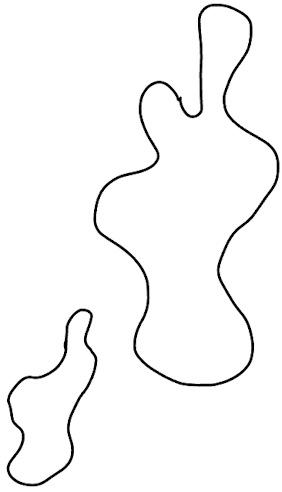
\includegraphics[width=.25\linewidth]{figure_source/polygon_reconstruction_1.png}
	\end{figure}
}
\only<2>{
	\begin{figure}
		\centering
		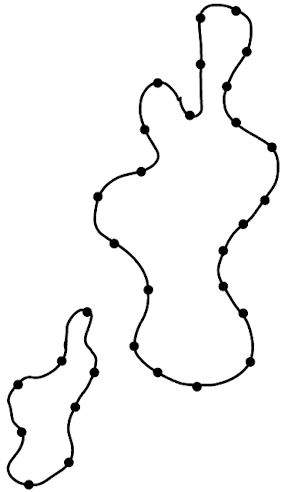
\includegraphics[width=.25\linewidth]{figure_source/polygon_reconstruction_2.png}
	\end{figure}
}
\only<3>{
	\begin{figure}
		\centering
		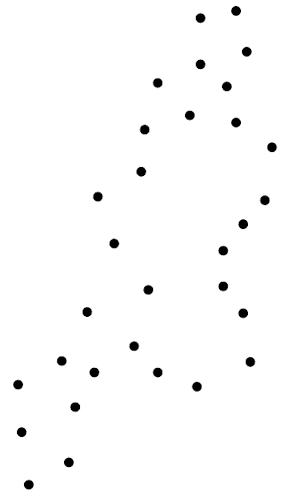
\includegraphics[width=.25\linewidth]{figure_source/polygon_reconstruction_3.png}
	\end{figure}
}
\only<4>{
	\begin{figure}
		\centering
		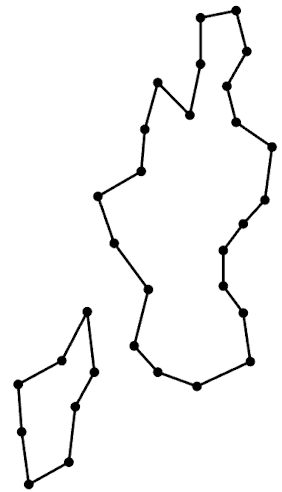
\includegraphics[width=.25\linewidth]{figure_source/polygon_reconstruction_4.png}
	\end{figure}
}

\end{frame}
